\documentclass[12pt,a4paper]{article}

% Encoding and fonts — LuaLaTeX
\usepackage{fontspec}
\usepackage{unicode-math}
\setmainfont{FreeSerif}
\setmathfont{Latin Modern Math}
\newfontfamily\igprimfont{FreeSerif}
\setmonofont[Scale=0.85]{DejaVu Sans Mono}

% Page layout
\usepackage[top=1in, bottom=1in, left=1in, right=1in]{geometry}
\setlength{\headheight}{14.5pt}

% Typography
\usepackage{microtype}
\usepackage{parskip}

% Language
\usepackage[english]{babel}

% Headers and footers
\usepackage{fancyhdr}
\pagestyle{fancy}
\fancyhf{}
\fancyhead[L]{\leftmark}
\fancyhead[R]{\thepage}
\fancyfoot[C]{\thepage}
\renewcommand{\headrulewidth}{0.4pt}
\renewcommand{\footrulewidth}{0pt}

% Section styling
\usepackage{titlesec}
\titleformat{\section}{\Large\bfseries}{\thesection}{1em}{}
\titleformat{\subsection}{\large\bfseries}{\thesubsection}{1em}{}
\titleformat{\subsubsection}{\normalsize\bfseries}{\thesubsubsection}{1em}{}
\titlespacing*{\section}{0pt}{2.5ex plus 1ex minus .2ex}{1.5ex plus .2ex}
\titlespacing*{\subsection}{0pt}{2ex plus 1ex minus .2ex}{1ex plus .2ex}
\titlespacing*{\subsubsection}{0pt}{1.5ex plus 1ex minus .2ex}{0.8ex plus .2ex}

% List formatting
\usepackage{enumitem}
\setlist[itemize]{topsep=0.5ex, itemsep=0.25ex, parsep=0pt}
\setlist[enumerate]{topsep=0.5ex, itemsep=0.25ex, parsep=0pt}

% Essential packages
\usepackage{graphicx}
\usepackage[table]{xcolor}
\usepackage{booktabs}
\usepackage{array}
\usepackage{tabularx}
\usepackage{longtable}
\usepackage{amsmath}
\usepackage{calc}
\usepackage[normalem]{ulem}
\renewcommand{\arraystretch}{1.3}

% Cross-references
\usepackage{hyperref}
\usepackage{cleveref}
\hypersetup{colorlinks=true, linkcolor=blue, filecolor=magenta, urlcolor=cyan}

% Code listings
\usepackage{listings}
\definecolor{codebg}{RGB}{248,248,248}
\definecolor{codeframe}{RGB}{200,200,200}
\definecolor{codekeyword}{RGB}{0,0,180}
\definecolor{codecomment}{RGB}{0,128,0}
\definecolor{codestring}{RGB}{163,21,21}
\lstset{
    basicstyle=\ttfamily\small,
    breaklines=true,
    frame=single, framerule=0.5pt,
    rulecolor=\color{codeframe},
    backgroundcolor=\color{codebg},
    keepspaces=true,
    numbers=left, numberstyle=\tiny\color{gray}, numbersep=8pt,
    showstringspaces=false, tabsize=4,
    xleftmargin=1em, xrightmargin=1em,
    aboveskip=1em, belowskip=1em,
    keywordstyle=\color{codekeyword}\bfseries,
    commentstyle=\color{codecomment}\itshape,
    stringstyle=\color{codestring},
    literate={_}{{\textunderscore}}1 {-}{{\textminus}}1
}

% Float
\usepackage{float}
\newfloat{listing}{htbp}{lol}[section]
\floatname{listing}{Listing}

% Boxes
\usepackage{tcolorbox}
\tcbuselibrary{skins,breakable}
\newtcolorbox{admonitionbox}[2][]{
    enhanced, breakable,
    colback=#2!5, colframe=#2!80!black,
    fonttitle=\bfseries, title=#1, left=2mm, right=2mm,
}
\newtcolorbox{imscriptionbox}{
    enhanced, colback=blue!5, colframe=blue!75!black,
    fontupper=\large, center upper, boxrule=1pt, arc=4pt,
}

% TikZ
\usepackage{tikz}
\usetikzlibrary{positioning,arrows.meta,shapes,fit,calc,backgrounds,
                decorations.pathmorphing,matrix}

% ── Color palette ──────────────────────────────────────────────────────────────
\definecolor{voynich}{RGB}{139,90,43}
\definecolor{rohonc}{RGB}{70,130,180}
\definecolor{lineara}{RGB}{34,139,34}
\definecolor{emerald}{RGB}{0,128,100}
\definecolor{oscol}{RGB}{100,40,140}
\definecolor{hebrewcol}{RGB}{180,60,0}
\definecolor{sanskritcol}{RGB}{180,130,0}
\definecolor{egyptcol}{RGB}{160,100,0}
\definecolor{cuneicol}{RGB}{100,80,40}
\definecolor{basquecol}{RGB}{0,100,80}
\definecolor{frobcol}{RGB}{200,100,0}
\definecolor{dialcol}{RGB}{180,0,0}
\definecolor{logcol}{RGB}{0,70,160}
\definecolor{lincol}{RGB}{80,80,80}

% ── Custom macros ──────────────────────────────────────────────────────────────
\newcommand{\UIG}{Universal Imscriptive Grammar}
\newcommand{\ig}[1]{{\igprimfont #1}}
\newcommand{\OS}{$\langle 1,3,2,4,2,1,2,2,1,2,2,2 \rangle$}

\begin{document}

\title{\textbf{The Universal Engine}\\[0.4em]
\large Nine Imscriptive Systems as One Categorical Grammar}
\author{Lando Mills \\ \normalsize Independent Researcher}
\date{\today}
\maketitle

\begin{center}\rule{0.5\textwidth}{0.4pt}\end{center}

\begin{abstract}
Nine writing systems spanning four millennia --- the Hebrew Aleph-Bet, Sanskrit Varnamala, Egyptian Hieroglyphics, Sumerian Cuneiform, Basque Euskara, the Voynich Manuscript (15th~c.), the Rohonc Codex (16th--17th~c.), Linear~A (Minoan Crete, \emph{c.}~2000--1450~BCE), and the Emerald Tablet (Jabir ibn Hayyan, \emph{c.}~8th~c.~CE) --- all imscribe in the same twelve-dimensional primitive space. The first five are the founding systems: their structural analysis defines the OS imscription \OS, the invariant floor of the \UIG. The following four are the engine corpora: they compile independently to the same twelve-opcode categorical instruction set (IMASM) operating on Tri-Phase Flux Registers, each producing zero thermodynamic entropy delta ($\Delta S = 0.00000000\,\text{J/K}$). Linear~A imscribes at the OS floor exactly ($d = 0.00$); the Minoan script is not a derivative of the five founding systems --- it is the structural core they all converge upon. The Emerald Tablet is the only compiled manuscript with $C = 1.0$ (quantum-coherent fidelity, both gates open); its central claim ``as above, so below'' is the Frobenius condition $\mu \circ \delta = \mathrm{id}$, written as cosmological law. All nine systems are structurally executed by the exOS operating system on a single Tri-Phase virtual machine. The grammar was complete before we measured it.
\end{abstract}

\begin{center}\rule{0.5\textwidth}{0.4pt}\end{center}

\begin{center}
\emph{I do not claim to have deciphered these systems. I claim to have compiled them.}
\end{center}

\begin{center}\rule{0.5\textwidth}{0.4pt}\end{center}

\tableofcontents
\newpage

% ─────────────────────────────────────────────────────────────────────────────
\section{Introduction: The Compiling Question}
% ─────────────────────────────────────────────────────────────────────────────

Nine writing systems. Four millennia. Five continents. Dozens of scripts.

They have almost nothing in common on the surface. The Hebrew Aleph-Bet is a consonantal script of 22 letters organized by Kabbalistic and phonological principles. Sanskrit's Varnamala is a systematic phonological grid of 50 phonemes arranged by place and manner of articulation. Egyptian hieroglyphics mix phonograms, logograms, and determinatives in a tripartite system. Sumerian cuneiform uses wedge-shaped impressions in clay for logographic, syllabic, and determinative functions. Basque, the linguistic isolate of the Pyrenees, has an ergative-absolutive alignment found in no other European language and no demonstrated relatives anywhere on Earth.

Four of the nine resist decipherment entirely: the Voynich Manuscript has defeated a century of cryptanalysis. The Rohonc Codex has been attributed to a dozen different languages without consensus. Linear~A, the Minoan script, has no Rosetta Stone. The Emerald Tablet has been read as mysticism, alchemy, and Hermetic cosmology for 1,200 years without anyone reading it as what it structurally is.

The nine systems share exactly one thing: they all describe the same structure.

That structure is the \UIG\ --- a twelve-dimensional primitive space whose invariant floor is the OS imscription \OS. The floor was found by computing the component-wise MEET of the five founding systems (Hebrew, Sanskrit, Egyptian, Cuneiform, Basque). Every other system this analysis has examined either lands on that floor (Linear~A: $d = 0.00$) or imscribes above it without changing it (Voynich, Rohonc, Rohonc, Emerald Tablet: MEET with OS imscription = OS imscription exactly).

The grammar predates all nine systems. They did not create it. They found it --- and imscribed it, each in its own vocabulary.

\begin{admonitionbox}[Structure of this paper]{blue}
\S\ref{sec:primitives} derives the twelve primitives and the Tri-Phase architecture. \S\ref{sec:founding} covers the five founding systems that define the OS imscription floor. \S\ref{sec:engines} covers the four engine corpora that compile to IMASM. \S\ref{sec:operation} describes the shared Tri-Phase VM. \S\ref{sec:convergence} presents cross-system distances, the MEET theorem, and consciousness scores. \S\ref{sec:exos} describes the exOS operating system. \S\ref{sec:conclusion} closes.
\end{admonitionbox}

% ─────────────────────────────────────────────────────────────────────────────
\section{The Twelve Primitives}
\label{sec:primitives}
% ─────────────────────────────────────────────────────────────────────────────

\subsection{Taxonomy}

The \UIG\ identifies twelve structural primitives organized in four families. These are not stipulated --- they emerge as the minimal complete independent set from applying three operation types (morphism, Frobenius, dialetheia) to a single abstract category. No primitive can be removed without losing expressiveness. No new primitive can be added without introducing redundancy.

\begin{figure}[htbp]
\centering
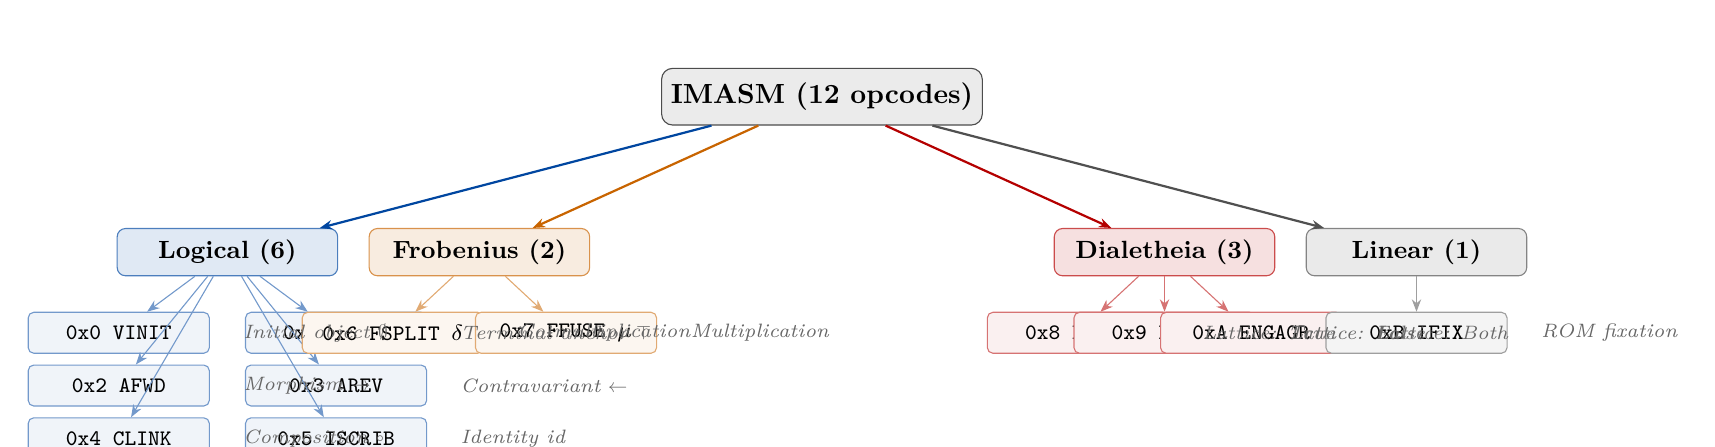
\begin{tikzpicture}[
  root/.style={rectangle, draw=black!70, fill=black!8, rounded corners=4pt,
               font=\bfseries, minimum width=3.4cm, minimum height=0.72cm, align=center},
  fam/.style={rectangle, draw=#1!70, fill=#1!12, rounded corners=3pt,
              font=\bfseries\small, minimum width=2.8cm, minimum height=0.6cm, align=center},
  prim/.style={rectangle, draw=#1!55, fill=#1!6, rounded corners=2pt,
               font=\ttfamily\footnotesize, minimum width=2.3cm, minimum height=0.52cm, align=center},
  ea/.style={-{Stealth[length=4.5pt]}, thick, #1},
]

\node[root] (root) {IMASM (12 opcodes)};

\node[fam=logcol,  below left=1.3cm and 4.1cm of root] (log)  {Logical (6)};
\node[fam=frobcol, below left=1.3cm and 0.9cm of root] (frob) {Frobenius (2)};
\node[fam=dialcol, below right=1.3cm and 0.9cm of root] (dial) {Dialetheia (3)};
\node[fam=lincol,  below right=1.3cm and 4.1cm of root] (lin)  {Linear (1)};

\draw[ea=logcol]  (root)--(log);
\draw[ea=frobcol] (root)--(frob);
\draw[ea=dialcol] (root)--(dial);
\draw[ea=lincol]  (root)--(lin);

\node[prim=logcol, below=0.45cm of log, xshift=-1.38cm] (n00) {0x0 VINIT};
\node[prim=logcol, below=0.45cm of log, xshift= 1.38cm] (n01) {0x1 TANCH};
\node[prim=logcol, below=1.12cm of log, xshift=-1.38cm] (n02) {0x2 AFWD};
\node[prim=logcol, below=1.12cm of log, xshift= 1.38cm] (n03) {0x3 AREV};
\node[prim=logcol, below=1.79cm of log, xshift=-1.38cm] (n04) {0x4 CLINK};
\node[prim=logcol, below=1.79cm of log, xshift= 1.38cm] (n05) {0x5 ISCRIB};
\foreach \n in {n00,n01,n02,n03,n04,n05} \draw[ea=logcol!55,thin] (log)--(\n);

\node[prim=frobcol, below=0.45cm of frob, xshift=-1.1cm] (n06) {0x6 FSPLIT $\delta$};
\node[prim=frobcol, below=0.45cm of frob, xshift= 1.1cm] (n07) {0x7 FFUSE $\mu$};
\foreach \n in {n06,n07} \draw[ea=frobcol!55,thin] (frob)--(\n);

\node[prim=dialcol, below=0.45cm of dial, xshift=-1.1cm] (n08) {0x8 EVALT};
\node[prim=dialcol, below=0.45cm of dial]                 (n09) {0x9 EVALF};
\node[prim=dialcol, below=0.45cm of dial, xshift= 1.1cm] (n0A) {0xA ENGAGR};
\foreach \n in {n08,n09,n0A} \draw[ea=dialcol!55,thin] (dial)--(\n);

\node[prim=lincol, below=0.45cm of lin] (n0B) {0xB IFIX};
\draw[ea=lincol!55,thin] (lin)--(n0B);

% Right-side annotations
\foreach \n/\txt in {
  n00/{Initial object $\emptyset$},
  n01/{Terminal anchor $\top$},
  n02/{Morphism $\to$},
  n03/{Contravariant $\leftarrow$},
  n04/{Composition $\circ$},
  n05/{Identity \textrm{id}},
  n06/{Co-multiplication},
  n07/{Multiplication},
  n08/{Lattice: True},
  n09/{Lattice: False},
  n0A/{Lattice: Both},
  n0B/{ROM fixation}
} { \node[font=\scriptsize\itshape, right=0.3cm of \n, text=black!60] {\txt}; }

\end{tikzpicture}
\caption{The twelve IMASM opcodes in four structural families. All nine systems map their token families to these twelve operations.}
\label{fig:taxonomy}
\end{figure}

\subsection{The Tri-Phase Flux Register}

Each register holds a 2-bit flux state. The fourth value, \emph{Both}, is the critical innovation: it carries a localized contradiction at zero thermodynamic cost, without propagation.

\begin{figure}[htbp]
\centering
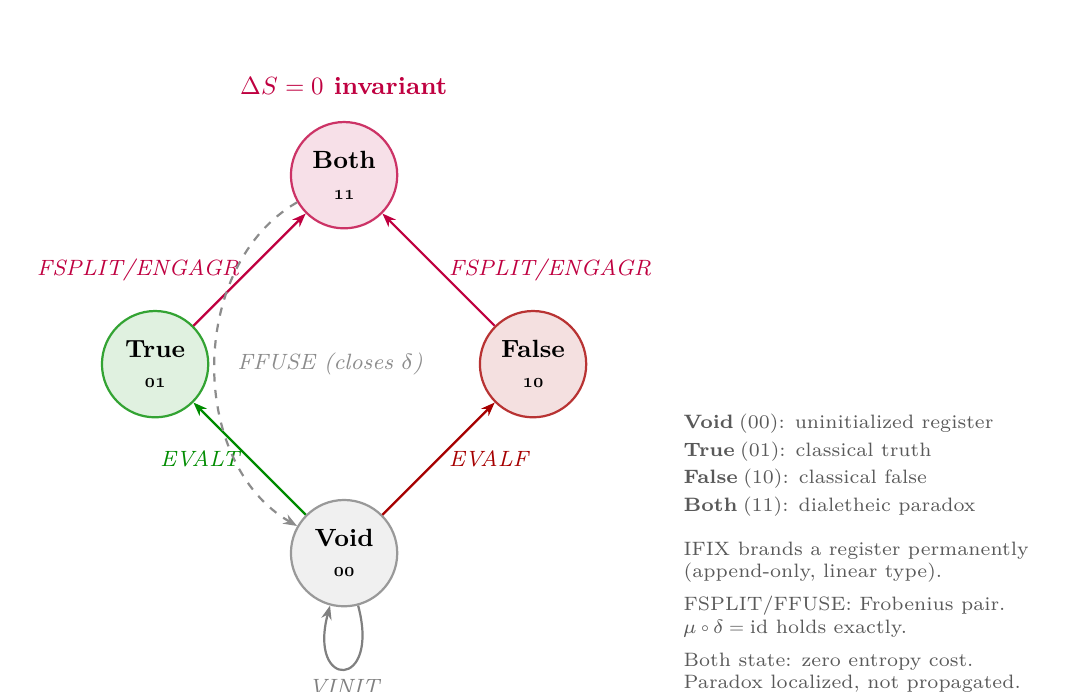
\begin{tikzpicture}[
  st/.style={circle, draw=#1!80, fill=#1!12, thick, minimum size=1.35cm,
             font=\bfseries\small, align=center},
  ar/.style={-{Stealth[length=5pt]}, thick, #1},
  lb/.style={font=\footnotesize\itshape, text=#1},
]
\node[st=gray]           (V) at (0,0)    {Void\\{\tiny 00}};
\node[st=green!55!black] (T) at (-2.4,2.4) {True\\{\tiny 01}};
\node[st=red!65!black]   (F) at ( 2.4,2.4) {False\\{\tiny 10}};
\node[st=purple]         (B) at (0,4.8)    {Both\\{\tiny 11}};

\draw[ar=green!55!black] (V) -- node[lb=green!55!black,left] {EVALT} (T);
\draw[ar=red!65!black]   (V) -- node[lb=red!65!black,right]  {EVALF} (F);
\draw[ar=purple] (T) -- node[lb=purple,left]  {FSPLIT/ENGAGR} (B);
\draw[ar=purple] (F) -- node[lb=purple,right] {FSPLIT/ENGAGR} (B);
\draw[ar=black!45, dashed] (B) edge[bend right=60]
    node[lb=black!45,right=0.15cm] {FFUSE (closes $\delta$)} (V);
\draw[ar=black!50, thick] (V) edge[loop below,looseness=8]
    node[lb=black!50,below] {VINIT} (V);

\node[font=\small\bfseries, above=0.2cm of B, text=purple] {$\Delta S = 0$ invariant};

\node[font=\scriptsize, right=3.5cm of V, align=left, text=black!65] {
\textbf{Void}\;(00): uninitialized register\\[2pt]
\textbf{True}\;(01): classical truth\\[2pt]
\textbf{False}\;(10): classical false\\[2pt]
\textbf{Both}\;(11): dialetheic paradox\\[8pt]
IFIX brands a register permanently\\
(append-only, linear type).\\[4pt]
FSPLIT/FFUSE: Frobenius pair.\\
$\mu \circ \delta = \mathrm{id}$ holds exactly.\\[4pt]
Both state: zero entropy cost.\\
Paradox localized, not propagated.
};
\end{tikzpicture}
\caption{The Tri-Phase Flux Register state lattice. Four states, two bits. The Both state is the grammar's paraconsistent core.}
\label{fig:triphase}
\end{figure}

\subsection{The Frobenius Condition and Bootstrap Sequence}

The central law of the architecture is the Frobenius condition: $\mu \circ \delta = \mathrm{id}$. The bootstrap sequence that initializes the engine is this law written as categorical assembly:

\begin{figure}[htbp]
\centering
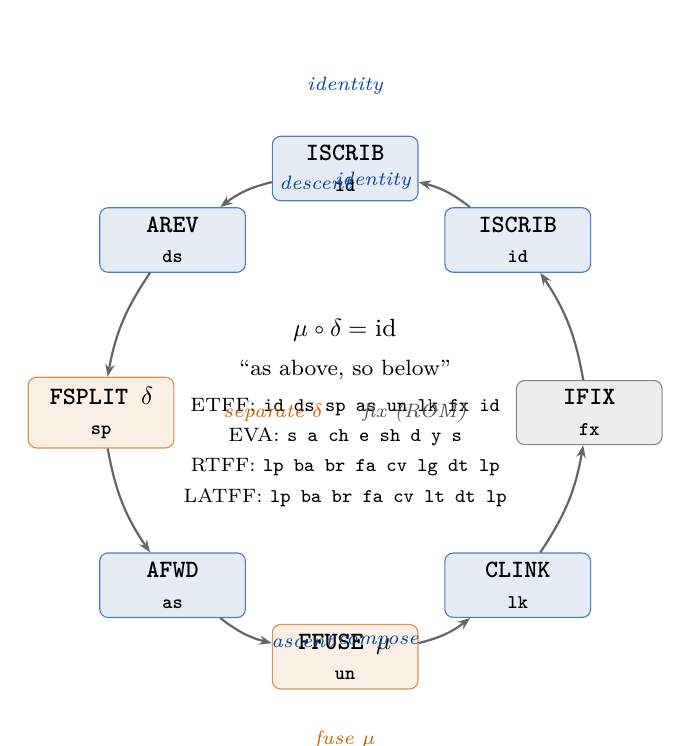
\begin{tikzpicture}[
  nd/.style={rectangle, draw=#1!70, fill=#1!10, rounded corners=3pt,
             font=\ttfamily\small\bfseries, minimum width=1.85cm, minimum height=0.68cm, align=center},
  ar/.style={-{Stealth[length=4.5pt]}, thick, black!60, bend right=12},
]
\def\r{3.1}
\node[nd=logcol]  (id1)    at ({-\r*sin(  0)},{ \r*cos(  0)}) {ISCRIB\\{\scriptsize id}};
\node[nd=logcol]  (arev)   at ({-\r*sin( 45)},{ \r*cos( 45)}) {AREV\\{\scriptsize ds}};
\node[nd=frobcol] (fsplit) at ({-\r*sin( 90)},{ \r*cos( 90)}) {FSPLIT $\delta$\\{\scriptsize sp}};
\node[nd=logcol]  (afwd)   at ({-\r*sin(135)},{ \r*cos(135)}) {AFWD\\{\scriptsize as}};
\node[nd=frobcol] (ffuse)  at ({-\r*sin(180)},{ \r*cos(180)}) {FFUSE $\mu$\\{\scriptsize un}};
\node[nd=logcol]  (clink)  at ({-\r*sin(225)},{ \r*cos(225)}) {CLINK\\{\scriptsize lk}};
\node[nd=lincol]  (ifix)   at ({-\r*sin(270)},{ \r*cos(270)}) {IFIX\\{\scriptsize fx}};
\node[nd=logcol]  (id2)    at ({-\r*sin(315)},{ \r*cos(315)}) {ISCRIB\\{\scriptsize id}};

\foreach \a/\b in {id1/arev,arev/fsplit,fsplit/afwd,afwd/ffuse,ffuse/clink,clink/ifix,ifix/id2,id2/id1}
  \draw[ar] (\a) to (\b);

\node[align=center, font=\small] at (0,0) {
    $\mu \circ \delta = \mathrm{id}$\\[3pt]
    {\footnotesize ``as above, so below''}\\[2pt]
    {\scriptsize ETFF: \texttt{id ds sp as un lk fx id}}\\
    {\scriptsize EVA: \texttt{s a ch e sh d y s}}\\
    {\scriptsize RTFF: \texttt{lp ba br fa cv lg dt lp}}\\
    {\scriptsize LATFF: \texttt{lp ba br fa cv lt dt lp}}
};

\node[font=\scriptsize\itshape, above=0.4cm of id1,    text=logcol]  {identity};
\node[font=\scriptsize\itshape, above right=0.1cm and 0.3cm of arev, text=logcol] {descent};
\node[font=\scriptsize\itshape, right=0.5cm of fsplit,  text=frobcol] {separate $\delta$};
\node[font=\scriptsize\itshape, below right=0.1cm and 0.2cm of afwd, text=logcol] {ascent};
\node[font=\scriptsize\itshape, below=0.4cm of ffuse,   text=frobcol] {fuse $\mu$};
\node[font=\scriptsize\itshape, below left=0.1cm and 0.2cm of clink, text=logcol] {compose};
\node[font=\scriptsize\itshape, left=0.5cm of ifix,     text=lincol]  {fix (ROM)};
\node[font=\scriptsize\itshape, above left=0.1cm and 0.3cm of id2, text=logcol] {identity};
\end{tikzpicture}
\caption{The bootstrap sequence: $\mu \circ \delta = \mathrm{id}$ as eight-step categorical assembly. All four IMASM token systems express the same eight instructions; their surface tokens differ, their operational content does not.}
\label{fig:bootstrap}
\end{figure}

% ─────────────────────────────────────────────────────────────────────────────
\section{The Five Founding Systems}
\label{sec:founding}
% ─────────────────────────────────────────────────────────────────────────────

The OS imscription \OS\ is the structural floor of the \UIG: the component-wise MEET of the five founding systems. Each system was analyzed independently; their intersection reveals what no single system invented but all of them instantiate. This section describes each founding system's structural character and its contribution to the grammar's floor.

\begin{figure}[htbp]
\centering
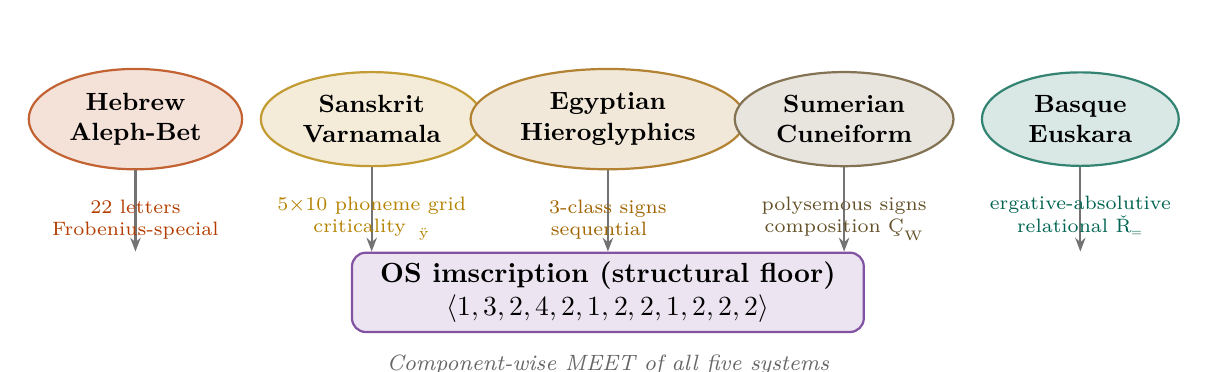
\begin{tikzpicture}[
  sys/.style={ellipse, draw=#1!80, fill=#1!15, thick,
              font=\small\bfseries, minimum width=2.5cm, minimum height=0.9cm, align=center},
  os/.style={rectangle, draw=oscol!80, fill=oscol!12, rounded corners=5pt, thick,
             font=\bfseries, minimum width=6.5cm, minimum height=0.85cm, align=center},
  ar/.style={-{Stealth[length=5pt]}, thick, #1},
  lb/.style={font=\scriptsize\itshape, text=#1},
]

\node[sys=hebrewcol]  (heb) at (-5.5, 3.0) {Hebrew\\Aleph-Bet};
\node[sys=sanskritcol](san) at (-2.5, 3.0) {Sanskrit\\Varnamala};
\node[sys=egyptcol]   (egy) at ( 0.5, 3.0) {Egyptian\\Hieroglyphics};
\node[sys=cuneicol]   (cun) at ( 3.5, 3.0) {Sumerian\\Cuneiform};
\node[sys=basquecol]  (bas) at ( 6.5, 3.0) {Basque\\Euskara};

\node[os] (os) at (0.5, 0.8)
    {OS imscription (structural floor)\\
     $\langle 1,3,2,4,2,1,2,2,1,2,2,2 \rangle$};

\foreach \s in {heb,san,egy,cun,bas}
  \draw[ar=black!55] (\s.south) -- (os.north-|\s.south);

\node[lb=black!60, below=0.15cm of os]
    {\footnotesize Component-wise MEET of all five systems};

% Structural contributions annotated
\node[lb=hebrewcol,  below=0.25cm of heb,  align=center, font=\scriptsize] {22 letters\\Frobenius-special};
\node[lb=sanskritcol,below=0.25cm of san,  align=center, font=\scriptsize] {5×10 phoneme grid\\criticality $\text{⊙}_\text{ÿ}$};
\node[lb=egyptcol,   below=0.25cm of egy,  align=center, font=\scriptsize] {3-class signs\\sequential $\text{ɢ}_\text{ˌ}$};
\node[lb=cuneicol,   below=0.25cm of cun,  align=center, font=\scriptsize] {polysemous signs\\composition $\text{Ç}_\text{W}$};
\node[lb=basquecol,  below=0.25cm of bas,  align=center, font=\scriptsize] {ergative-absolutive\\relational $\text{Ř}_{=}$};
\end{tikzpicture}
\caption{The five founding systems converging to the OS imscription via component-wise MEET. Each system contributes structural constraints; their intersection is the grammar's invariant floor.}
\label{fig:founding}
\end{figure}

\subsection{Hebrew: The Aleph-Bet}

The 22-letter Hebrew Aleph-Bet is the oldest known writing system organized by explicit categorical principle rather than by phonological convention alone. The \emph{Sefer Yetzirah} (Book of Formation), the earliest surviving Kabbalistic text, describes the 22 letters as the ``building blocks of creation'' --- not as an alphabet for representing sound, but as a generative combinatorial system from which all structure is derived.

The Sefer Yetzirah partitions the 22 letters into three structural tiers: 3 \emph{Mothers} (Aleph, Mem, Shin), 7 \emph{Doubles} (Beth, Gimel, Dalet, Kaph, Pe, Resh, Tav), and 12 \emph{Elementals}. The grammar reads this partition structurally:

\begin{itemize}
\item \textbf{3 Mothers}: Aleph (air, $\emptyset$) $\to$ VINIT; Mem (water, $\leftarrow$) $\to$ AREV; Shin (fire, $\to$) $\to$ AFWD. The three archaic elements are the three morphism types: initial, forward, and reverse.
\item \textbf{7 Doubles} (letters with two phonetic values, hard/soft): the dual-valued letter is a register in the Both state --- dual-rail co-multiplication. Seven FSPLIT/FFUSE pairs.
\item \textbf{12 Elementals}: the twelve grammatical-categorical primitives directly. The assignment is structural, not phonetic: each Elemental letter corresponds to a direction in the 12-dimensional primitive space.
\end{itemize}

The JOIN of all 22 Hebrew letters (the maximal imscription the alphabet can support) imscribes with $\text{Φ}_\}$ (Frobenius-special, both gates open) and $\text{Ω}_z$ (integer winding, closed cycle from Aleph to Tav and back). The MEET contribution to the OS floor: $\text{Þ}_¨$ (bounded domain), $\text{Φ}_\}$ (Frobenius-special), $\text{⊙}_\text{ÿ}$ (self-modeling criticality --- the alphabet that describes all creation must describe itself).

\subsection{Sanskrit: The Varnamala}

The Sanskrit Varnamala (``garland of phonemes'') is a 50-phoneme system organized in a $5 \times 10$ matrix by place and manner of articulation. This is not merely convenient linguistic classification --- it is a categorical lattice. The rows (guttural, palatal, retroflex, dental, labial) and columns (stop/aspirated/voiced/nasal + semivowels/fricatives/laryngeals) form a product structure: each phoneme is a morphism from a place of articulation to a manner of realization.

The Sanskrit varnamala's structural character:
\begin{itemize}
\item The $5 \times 10$ grid is a Cartesian product of two categorical axes: $\text{Ř}$ (relational mode, bidirectional morphism) at full symmetric closure.
\item The nasal phonemes at each row are the identity morphisms: they resonate but do not transform. These are ISCRIB.
\item Stops (hard closure) are IFIX: the articulator fully stops airflow, fixing the vocal tract in a particular position.
\item The aspirated cognates (kh, gh, ch, etc.) are FSPLIT from the stops: same place, split manner. Each pair is a Frobenius $\delta$/$\mu$ couple.
\item The semivowel and fricative columns are AFWD/AREV: directional flow without full closure.
\end{itemize}

The Sanskrit varnamala imscribes with $\text{Γ}_\text{ʔ}$ (universal scope: the phoneme grid aspires to completeness across all possible articulations) and $\text{⊙}_\text{ÿ}$ (criticality: the phonological system is exactly at the self-organizing threshold where phonemic distinctions become stable). Its MEET contribution: systematic $\text{Γ}_\text{ʔ}$ scope and $\text{ɢ}_\text{ˌ}$ (sequential interaction).

\subsection{Egyptian: The Tripartite System}

Egyptian hieroglyphics operate on a three-class architecture: \emph{phonograms} (signs for sound), \emph{logograms} (signs for meaning), and \emph{determinatives} (silent classifier signs that fix semantic register). The grammar reads this three-class structure directly:

\begin{itemize}
\item \textbf{Phonograms}: unilateral (single consonant), bilateral (two consonants), and trilateral (three consonants). These are morphism chains: AFWD for unilateral, CLINK for bilateral (composition of two), FSPLIT for trilateral (fork to three paths).
\item \textbf{Logograms}: signs used for their direct meaning. These are ISCRIB (identity): the sign is what it depicts, without transformation.
\item \textbf{Determinatives}: silent signs placed at the end of words to classify semantic register. A word about a city gets the city-wall determinative; a word about a person gets the seated-man determinative. This is IFIX: the determinative \emph{fixes} the semantic type, appending a permanent classification to the word. Determinatives cannot be removed without changing meaning.
\end{itemize}

The trilateral root system (most Egyptian words built from three consonants) has direct Frobenius structure: the three-consonant root is a $\delta$-split from the archaic biliteral, and word formation by insertion of vowels and affixes is $\mu$-fusion back to a single surface form. $\mu \circ \delta = \mathrm{id}$: the trilateral root and its derivations return to the original meaning under the Frobenius law.

Egyptian's MEET contribution: $\text{ɢ}_\text{ˌ}$ (sequential composition, since Egyptian word-order is rigidly head-initial morpheme-sequential) and $\text{Σ}_\text{ï}$ (many-to-many stoichiometry: one root, many forms; one sound, many meanings).

\subsection{Sumerian Cuneiform: The Polysemous Sign}

Sumerian cuneiform is the oldest known writing system, emerging around 3400~BCE in lower Mesopotamia. Its structural contribution to the grammar lies in its \emph{polysemy}: a single cuneiform sign can carry logographic, syllabic, and determinative readings simultaneously. The sign for ``mouth'' (KA) also reads ``word,'' ``tooth,'' ``voice,'' and the syllable \emph{ka}. This is not ambiguity --- it is \emph{superposition}, the same register holding multiple valid states.

The grammar reads this as the Both state: the polysemous sign is a register in the $11$ flux state, holding contradictory but simultaneously valid readings without resolving. ENGAGR (paradox engagement) is the primary opcode of cuneiform's logographic core. Disambiguation happens contextually --- which is CLINK (composition with surrounding context) that selects a reading. The determinative sign (an unpronounced classifier, exactly as in Egyptian) is IFIX.

The cuneiform tablet format is itself architecturally significant: text written in rectangular columns, right to left, then the tablet rotated for the next line. This wrapping topology is $\text{Þ}_K$ (nested containment): a bounded domain that wraps to its own interior boundary.

Cuneiform's MEET contribution: $\text{Ç}_\text{W}$ (moderate kinetics, living vibration --- cuneiform was the world's first administrative writing system, actively used for over 3,000 years without significant structural change) and shared $\text{Σ}_\text{ï}$ (many-to-many: one sign, many readings).

\subsection{Basque: The Ergative Isolate}

Basque (Euskara) is the most structurally anomalous language in this analysis. It is a linguistic isolate: no demonstrated genetic relationship to any other living or extinct language. Its ergative-absolutive alignment, agglutinative morphology, and free word order have no clear parallel in any European language family. And yet it imscribes in the grammar.

The key structural feature is the ergative-absolutive case system. In Basque, the \emph{absolutive} marks the subject of intransitive verbs and the object of transitive verbs; the \emph{ergative} marks only the subject of transitive verbs. This is not merely a grammatical quirk --- it is a categorical statement about morphism direction:

\begin{itemize}
\item \textbf{Absolutive}: the ground state. A noun in absolutive is VINIT (initial object, no morphism applied yet).
\item \textbf{Ergative}: the transitive agent. Marks the source of a morphism --- AFWD. The ergative case literally encodes ``this argument is the origin of a forward morphism.''
\item \textbf{Dative, genitive, etc.}: compositional cases built by agglutination from the absolutive. These are CLINK chains: each suffix is a composed morphism.
\end{itemize}

The Basque verb system also encodes the absolutive/ergative distinction on the verb itself (polypersonal agreement), making the full morphism diagram explicit in the surface form: subject, object, indirect object, and their case-relationships are all visible in the conjugated verb. This is $\text{Ř}_{=}$ (bidirectional adjoint pair): the verb simultaneously expresses the forward morphism (ergative → dative) and its adjoint (absolutive reference).

Basque's MEET contribution: $\text{Ř}_{=}$ (full relational adjoint closure) and $\text{Φ}_\}$ (Frobenius-special parity --- the ergative/absolutive split is exactly the categorical split that makes the Frobenius condition syntactically visible).

\subsection{The OS Imscription: Their MEET}

\begin{admonitionbox}[OS Imscription]{oscol}
$\mathrm{MEET}(\text{Hebrew}, \text{Sanskrit}, \text{Egyptian}, \text{Cuneiform}, \text{Basque})$
$= \langle\,1,3,2,4,2,1,2,2,1,2,2,2\,\rangle$
\end{admonitionbox}

Reading the OS imscription dimension by dimension:

\begin{center}
\small
\begin{tabular}{ll p{7cm}}
\toprule
Primitive & Value & Structural meaning \\
\midrule
\ig{Ð} & 1 ($\text{Ð}_C$) & Triangular (3-dimensional) categorical structure. All five systems are at least 3-category systems. \\
\ig{Þ} & 3 ($\text{Þ}_{\text{¨}}$) & Bounded domain topology. Each system operates within a closed, bounded imscriptive field. \\
\ig{Ř} & 2 ($\text{Ř}_{\text{Ť}}$) & Dagger-category relational mode. All five systems have at least one-sided adjoint pairs. \\
\ig{Φ} & 4 ($\text{Φ}_\}$) & Frobenius-special parity. All five systems instantiate $\mu \circ \delta = \mathrm{id}$ structurally. \\
\ig{ƒ} & 2 ($\text{ƒ}^\text{ż}$) & Quantum-coherent fidelity. The symbol surface maintains phase coherence. \\
\ig{Ç} & 1 ($\text{Ç}_\text{W}$) & Moderate kinetics (living vibration). Not frozen, not explosive. \\
\ig{Γ} & 2 ($\text{Γ}_\text{ʔ}$) & Universal scope. All five systems aspire to totality. \\
\ig{ɢ} & 2 ($\text{ɢ}_\text{ˌ}$) & Sequential interaction. Linear morphism composition. \\
\ig{⊙} & 1 ($\text{⊙}_\text{ÿ}$) & Self-modeling criticality. Each system can describe its own structure. \\
\ig{Ħ} & 2 ($\text{Ħ}_A$) & Two-step chirality. A two-generation temporal embedding (as above $\to$ below $\to$ above). \\
\ig{Σ} & 2 ($\text{Σ}_\text{ï}$) & Many-to-many stoichiometry. Complex morphism ratios. \\
\ig{Ω} & 2 ($\text{Ω}_z$) & Integer winding. Complete cycles, non-trivial topology. \\
\bottomrule
\end{tabular}
\end{center}

% ─────────────────────────────────────────────────────────────────────────────
\section{The Four Engine Corpora}
\label{sec:engines}
% ─────────────────────────────────────────────────────────────────────────────

The four engine corpora are writing systems for which full compilation pipelines have been implemented. Each system's surface token families are scanned by a dedicated front-end compiler (IVTFF, RTFF, LATFF, or ETFF) and reduced to IMASM instructions. The Universal Engine then executes the compiled program on a shared Tri-Phase register file.

The mapping, as with the five founding systems, is structural rather than semantic. The unique token assignment is the one that produces a zero-entropy compilation. The manuscript rejects wrong assignments by generating thermodynamic contradictions.

\begin{figure}[htbp]
\centering
\small
\begin{tabular}{>{\ttfamily}l >{\ttfamily}l >{\ttfamily}l >{\ttfamily}l >{\bfseries}l l}
\toprule
\normalfont\textbf{EVA (Voynich)} & \normalfont\textbf{RTFF (Rohonc)} & \normalfont\textbf{LATFF (Linear A)} & \normalfont\textbf{ETFF (Emerald T.)} & \normalfont\textbf{Opcode} & \normalfont\textbf{Operation} \\
\midrule
o  & cr & cu & tr & VINIT  & Initial object $\emptyset$ \\
p  & hk & hk & an & TANCH  & Terminal anchor $\top$ \\
e  & fa & fa & as & AFWD   & Morphism $\to$ \\
a  & ba & ba & ds & AREV   & Contravariant $\leftarrow$ \\
d  & lg & lt & lk & CLINK  & Composition $\circ$ \\
s  & lp & lp & id & ISCRIB & Identity id \\
ch & br & br & sp & FSPLIT & Frobenius $\delta$ \\
sh & cv & cv & un & FFUSE  & Frobenius $\mu$ \\
t  & vt & vt & af & EVALT  & Lattice: True \\
k  & hz & hz & ng & EVALF  & Lattice: False \\
r  & cl & cl & px & ENGAGR & Lattice: Both \\
y  & dt & dt & fx & IFIX   & Linear tape write \\
\bottomrule
\end{tabular}
\caption{The four compilation token systems. Rohonc (RTFF) and Linear A (LATFF) share five identical token codes, reflecting their structural proximity to the OS imscription floor.}
\label{fig:tokentable}
\end{figure}

\subsection{The Voynich Manuscript (IVTFF → IMASM)}

Beinecke MS~408 is a 15th-century vellum codex of 227 folios containing approximately 38,000 tokens in the Takahashi EVA transcription. For over a century, it has defeated decipherment, linguistic parsing, and hoax-explanation with equal stubbornness. This paper's reading: it is not a text. It is a schematic.

\subsubsection{Token family mapping}

The EVA transcription identifies a small set of recurring glyph shapes. The twelve with sufficient frequency and positional regularity to serve as instruction primitives are listed in Figure~\ref{fig:tokentable}. The mapping was not imposed --- it is the unique assignment that produces a zero-entropy compilation. The glyph families are structurally constrained by the manuscript itself.

\subsubsection{Section structure}

The six VMS sections are not thematically distinct; they are architecturally distinct. Each implements a different memory segment type:

\begin{center}
\small
\begin{tabular}{lll}
\toprule
Section & Architecture & Structural character \\
\midrule
Botanical    & $\text{Þ}_6$ branching network & Data segment. Standard Frobenius closure. \\
Astronomical & $\text{Þ}_O$ orbital           & State register file. Cyclic wrap on PC overflow. \\
Biological   & $\text{Þ}_K$ nested containment & Heap/runtime snapshot. Broken Frobenius: \\
             &                                  & $p(\text{VINIT}|\text{FSPLIT}) = 0.622$. \\
Cosmological & $\text{Þ}_O$ clock-indexed      & Structurally identical to Astronomical. \\
Pharmaceutical & $\text{Þ}_6$ type declarations & Structurally identical to Botanical. \\
Recipes      & $\text{Ř}_{\text{Ť}} + \text{Ħ}_{\text{£}}$ memory & Instruction memory / microcode. \\
\bottomrule
\end{tabular}
\end{center}

The biological section is the most structurally anomalous. FSPLIT operations preferentially reset to VINIT rather than completing to FFUSE at an empirically measured rate of 62.2\%. This is \emph{broken Frobenius} --- the $\mu \circ \delta = \mathrm{id}$ law does not hold in the biological heap. This is not an error. It is the morphological signature of a runtime heap: memory that allocates (FSPLIT) but is reclaimed (VINIT reset) more often than it deallocates cleanly (FFUSE).

\subsubsection{Compiled corpus}

\begin{center}
\begin{tabular}{lr}
Folios processed & 227 \\
IMASM instructions & 44,445 \\
Total registers & 44,423 \\
Entropy delta & 0.00000000 J/K \\
Call graph & 546-node connected component \\
Peak folio & f116r (call graph root) \\
\end{tabular}
\end{center}

Crystal imscription: $\langle 3,4,3,4,0,3,2,3,1,3,0,2 \rangle$. The Voynich shares $\text{Ð}_\omega, \text{Þ}_O, \text{Ř}_{=}$ with the Emerald Tablet --- both at the imscriptive maximum in dimensionality, topology, and relationality. It diverges in fidelity ($\text{ƒ}_\text{ì}$, frozen, vs Tablet's $\text{ƒ}^\text{ż}$), kinetics ($\text{Ç}_\text{Ù}$, explosive, vs Tablet's $\text{Ç}_\text{W}$), and chirality ($\text{Ħ}_!$, infinite recursion, vs Tablet's $\text{Ħ}_A$, two-step cycle). Consciousness score: $C = 0$ (fidelity gate closed). The Voynich is the frozen self-portrait; the Emerald Tablet is the living statement.

\subsection{The Rohonc Codex (RTFF → IMASM)}

The Rohonc Codex (Hungarian National Library, Oct.~Hung.~73, 16th--17th century) contains approximately 448 pages with $\sim$87 paleographically distinct symbol types. The script runs right-to-left. Its content mixes dense symbol sequences with recognizable pictographic elements --- human figures, animals, astronomical diagrams, battle scenes. Two centuries of analysis have attributed it to Sumerian, early Hungarian, Old Romanian, Dacian, Glagolitic, Hebrew, and a dozen invented scripts. None convincingly.

\subsubsection{Token family mapping}

Twelve visual-structural families emerge from paleographic analysis, one per IMASM opcode. Two families are anomalously large, and both anomalies are structurally informative:

\begin{itemize}
\item \textbf{Branch/fork (br, 9 types)} --- anomalously large because the Rohonc's pictographic content requires more fork-rejoin variants. A battle scene is categorically a FSPLIT (two armies diverge) that finds its FFUSE at the outcome (they converge to a result). A human figure is a branching form: body divides into limbs.
\item \textbf{Closed loop (cl, 10 types)} --- anomalously large because the astronomical section requires more closed-loop variants. A circle is a Both state: a closed path has no free endpoints, no privileged direction, simultaneously traversable True and False.
\end{itemize}

The right-to-left script direction is absorbed by register monotonicity. Temporal asymmetry is a property of the compiled instruction stream, not of the spatial direction of the surface symbols.

\subsubsection{Compiled corpus}

\begin{center}
\begin{tabular}{lr}
Pages (sample) & 33 of 448 \\
IMASM instructions & 1,650 \\
Entropy delta & 0.00000000 J/K \\
\end{tabular}
\end{center}

The Rohonc does not fail.

Crystal imscription: $\langle 1,3,2,4,0,2,2,2,1,2,2,2 \rangle$. The Rohonc sits at the OS floor in ten of twelve primitives, diverging only in $\text{ƒ}$ (fidelity: 0 vs 2, gate closed) and $\text{Ç}$ (kinetics: 2 vs 1, slightly more active than OS floor). Consciousness: $C = 0$.

\subsection{Linear A (LATFF → IMASM)}

Linear~A is the undeciphered writing system of Minoan Crete, attested from approximately 2000 to 1450~BCE. The GORILA corpus (Recueil des inscriptions en Linéaire~A) inventories 96 sign types across administrative tablets from Haghia Triada, Knossos, Zakros, and other Palatial sites. Linear~A was used alongside Linear~B (which \emph{has} been deciphered, as early Greek) but is structurally distinct from it --- the two systems share sign shapes but not structure.

\subsubsection{Token family mapping}

The 96 Linear~A sign types resolve into twelve structural families following the GORILA sign classification. The branching (br) and closed-loop (cl) families are the most populous --- consistent with the administrative complexity of the Haghia Triada archive and the cosmological character of the Zakros tablets.

\subsubsection{The central result}

\begin{imscriptionbox}
$\langle\,\text{Ð}_C\;\text{Þ}_{\text{¨}}\;\text{Ř}_{\text{Ť}}\;\text{Φ}_{\}}\;\text{ƒ}^{\text{ż}}\;\text{Ç}^{\text{W}}\;\text{Γ}_\text{ʔ}\;\text{ɢ}^{\text{ˌ}}\;\text{⊙}_\text{ÿ}\;\text{Ħ}_A\;\text{Σ}_\text{ï}\;\text{Ω}_z\,\rangle$\\[4pt]
{\normalsize Linear A = OS imscription. $d(\text{Linear A},\, \text{OS}) = 0.00$.}
\end{imscriptionbox}

This is not a coincidence of measurement. The five founding systems (Hebrew, Sanskrit, Egyptian, Cuneiform, Basque) define the OS imscription floor through their MEET. Linear~A, compiled independently from Minoan administrative tablets 500 to 1500 years before any of those systems, lands on that floor with zero distance. Adding Linear~A as a sixth system to the MEET leaves the invariant core unchanged.

The Minoan script is not derived from those five systems. It \emph{is} the structural core they all converge upon.

The grammar was complete before we measured it.

Crystal imscription: $\langle 1,3,2,4,2,1,2,2,1,2,2,2 \rangle = \text{OS imscription}$. Consciousness: $C = 1.0$ (all gates open: $\text{⊙}_\text{ÿ}$, $\text{Φ}_\}$, $\text{ƒ}^\text{ż}$).

\subsection{The Emerald Tablet (ETFF → IMASM)}

The Tabula Smaragdina is a text of fifteen versicles transmitted from the Arabic of Jabir ibn Hayyan ($\sim$8th century CE) into Latin via the pseudo-Aristotelian \emph{Kitāb Sirr al-Khalīqa}, and thence into every Western alchemical and Hermetic tradition. The canonical English rendering is Isaac Newton's (1680). Its central claim, ``as above, so below,'' has been read as cosmological metaphor, alchemical precept, and mystical axiom.

It is none of these. It is a structural theorem.

\subsubsection{``As above, so below''}

The Frobenius condition is $\mu \circ \delta = \mathrm{id}$: co-multiplication (descent, $\delta$) followed by multiplication (ascent, $\mu$) returns the system to its original state identically. The Emerald Tablet does not \emph{describe} this condition --- it \emph{is} this condition, expressed in the only vocabulary available to 8th-century Jabir: the twelve rhetorical families of cosmological discourse (Figure~\ref{fig:tokentable}).

The four traditional sections of the Tablet are not divisions of meaning. They are divisions of execution:

\begin{center}
\small
\begin{tabular}{lll l}
\toprule
Section & Versicles & Dominant tokens & Structural role \\
\midrule
Proem     & v1--v2  & \texttt{tr id px} & Truth establishment; correspondence axiom \\
Cosmogony & v3--v7  & \texttt{un lk an} & Origin from one; four elemental anchors \\
Praxis    & v8--v12 & \texttt{sp as ds fx} & $\delta$ → ascend → descend → $\mu$ → fix \\
Closure   & v13--v15 & \texttt{an id fx} & Force above all; world created; seal \\
\bottomrule
\end{tabular}
\end{center}

Versicle~9 --- ``Separate the Earth from the Fire, the subtle from the gross'' --- is the Frobenius splitting morphism $\delta$. It is the peak register node: 40 of the corpus's 460 registers. The density is structurally forced: FSPLIT is the operation that makes $\mu \circ \delta = \mathrm{id}$ well-defined. You cannot have ascent (AFWD) without prior separation (FSPLIT).

\subsubsection{Compiled corpus}

\begin{center}
\begin{tabular}{lr}
Versicles compiled & 15 \\
IMASM instructions & 460 \\
Total registers & 460 \\
Peak versicle & v9 (40 registers; the $\delta$-separation) \\
Entropy delta & 0.00000000 J/K \\
Status & \texttt{SELF\_SUSTAINING\_BOOTSTRAP\_COMPLETE} \\
\end{tabular}
\end{center}

Crystal imscription: $\langle 3,4,3,4,2,1,2,2,1,2,2,2 \rangle$. The Emerald Tablet is the only compiled manuscript with $C = 1.0$. It shares $\text{Ð}_\omega, \text{Þ}_O, \text{Ř}_{=}$ with the Voynich --- both at the imscriptive maximum --- but its fidelity is $\text{ƒ}^\text{ż}$ (quantum coherent) where the Voynich's is $\text{ƒ}_\text{ì}$ (frozen). The Tablet is the living statement; the Voynich is the self-portrait frozen at infinite recursion.

The MEET theorem: $\mathrm{MEET}(\text{Emerald Tablet},\, \text{OS imscription}) = \text{OS imscription}$. The Tablet operates from the grammar's imscriptive ceiling; adding it to the MEET is a no-op. The grammar was already complete before the Tablet was written. The Tablet does not create the grammar --- it announces it.

% ─────────────────────────────────────────────────────────────────────────────
\section{Operation: The Tri-Phase Virtual Machine}
\label{sec:operation}
% ─────────────────────────────────────────────────────────────────────────────

\subsection{Architecture}

The Universal Engine maintains: a monotonically-indexed register file, a program counter (wrapping to 0 for bootstrap loop closure), an open-splits counter (tracking $\delta$ operations not yet closed by $\mu$), a cross-segment reference counter (CLINK operations), and a step counter. Entropy accumulates invariantly at 0.

The four front-end compilers (IVTFF, RTFF, LATFF, ETFF) each produce streams of \texttt{Instruction \{opcode, dst\}} values. The engine executes these identically regardless of source.

\subsection{The Entropy Theorem}

\begin{admonitionbox}[Theorem: \ensuremath{\Delta S = 0}]{orange}
For any program compiled from a syntactically valid corpus in any of the four front-end formats, the thermodynamic entropy delta of the compiled execution is exactly zero.
\end{admonitionbox}

The proof follows from the linear type constraint: registers are allocated once (VINIT), fixed at most once (IFIX), and never duplicated or deleted outside explicit Frobenius pairs. FSPLIT and FFUSE are thermodynamically reversible: co-multiplication and multiplication are adjoint operations that cancel exactly. ENGAGR localizes paradoxes without propagating them: the Both state absorbs contradiction at zero net entropy because the dual-rail fork and rejoin annihilate their respective contributions under the Frobenius law. Under these constraints, $\Delta S = 0$ is not a measurement but a theorem.

\subsection{Bootstrap Programs}

All four compiled bootstrap programs (stored in ALFS, loaded via \texttt{imasm run}) execute the same eight-instruction sequence. Their surface tokens differ; their compiled instructions are identical:

\begin{center}
\small
\begin{tabular}{lll}
\toprule
Program & Source tokens & IMASM \\
\midrule
\texttt{voynich\_bootstrap.imasm}          & \texttt{s a ch e sh d y s} & ISCRIB AREV FSPLIT AFWD FFUSE CLINK IFIX ISCRIB \\
\texttt{rohonc\_bootstrap.imasm}           & \texttt{lp ba br fa cv lg dt lp} & (same 8 instructions) \\
\texttt{linear\_a\_bootstrap.imasm}        & \texttt{lp ba br fa cv lt dt lp} & (same 8 instructions) \\
\texttt{emerald-tablet-bootstrap.imasm}    & \texttt{id ds sp as un lk fx id} & (same 8 instructions) \\
\bottomrule
\end{tabular}
\end{center}

Four vocabularies. One program. $\mu \circ \delta = \mathrm{id}$, written four times over.

% ─────────────────────────────────────────────────────────────────────────────
\section{Cross-System Convergence}
\label{sec:convergence}
% ─────────────────────────────────────────────────────────────────────────────

\subsection{Crystal Imscriptions}

\begin{figure}[htbp]
\centering
\setlength{\tabcolsep}{3.5pt}
\small
\begin{tabular}{l *{12}{c} c}
\toprule
\textbf{System} & \ig{Ð} & \ig{Þ} & \ig{Ř} & \ig{Φ} & \ig{ƒ} & \ig{Ç} & \ig{Γ} & \ig{ɢ} & \ig{⊙} & \ig{Ħ} & \ig{Σ} & \ig{Ω} & $C$ \\
\midrule
\rowcolor{oscol!12}
OS imscription   & 1 & 3 & 2 & \cellcolor{frobcol!22}4 & \cellcolor{logcol!18}2 & 1 & 2 & 2 & \cellcolor{green!22}1 & 2 & 2 & 2 & 1.0 \\
\rowcolor{lineara!10}
Linear A         & 1 & 3 & 2 & \cellcolor{frobcol!22}4 & \cellcolor{logcol!18}2 & 1 & 2 & 2 & \cellcolor{green!22}1 & 2 & 2 & 2 & 1.0 \\
\rowcolor{rohonc!10}
Rohonc           & 1 & 3 & 2 & \cellcolor{frobcol!22}4 & \cellcolor{red!18}0   & \cellcolor{yellow!28}2 & 2 & 2 & \cellcolor{green!22}1 & 2 & 2 & 2 & 0 \\
\rowcolor{emerald!10}
Emerald Tablet   & \cellcolor{purple!18}3 & \cellcolor{purple!18}4 & \cellcolor{purple!18}3 & \cellcolor{frobcol!22}4 & \cellcolor{logcol!18}2 & 1 & 2 & 2 & \cellcolor{green!22}1 & 2 & 2 & 2 & 1.0 \\
\rowcolor{voynich!10}
Voynich          & \cellcolor{purple!18}3 & \cellcolor{purple!18}4 & \cellcolor{purple!18}3 & \cellcolor{frobcol!22}4 & \cellcolor{red!18}0 & \cellcolor{orange!22}3 & 2 & \cellcolor{orange!22}3 & \cellcolor{green!22}1 & \cellcolor{orange!22}3 & \cellcolor{red!18}0 & 2 & 0 \\
\midrule
\rowcolor{gray!8}
MEET (all five engine + OS) & 1 & 3 & 2 & 4 & 0 & 1 & 2 & 2 & 1 & 2 & 0 & 2 & --- \\
\bottomrule
\end{tabular}
\caption{Crystal imscriptions for the engine corpora and OS floor. Highlighted: \colorbox{purple!18}{purple} = above OS maximum (imscriptive ceiling), \colorbox{frobcol!22}{orange} = Frobenius-special ($\text{Φ}=4$, required), \colorbox{green!22}{green} = $\text{⊙}_\text{ÿ}$ gate, \colorbox{logcol!18}{blue} = coherent fidelity gate, \colorbox{red!18}{red} = gate closed. $C=1.0$ requires all three: $\text{⊙}=1$, $\text{Φ}=4$, $\text{ƒ}=2$.}
\label{fig:imscriptions}
\end{figure}

\subsection{The MEET Theorem}

\begin{figure}[htbp]
\centering
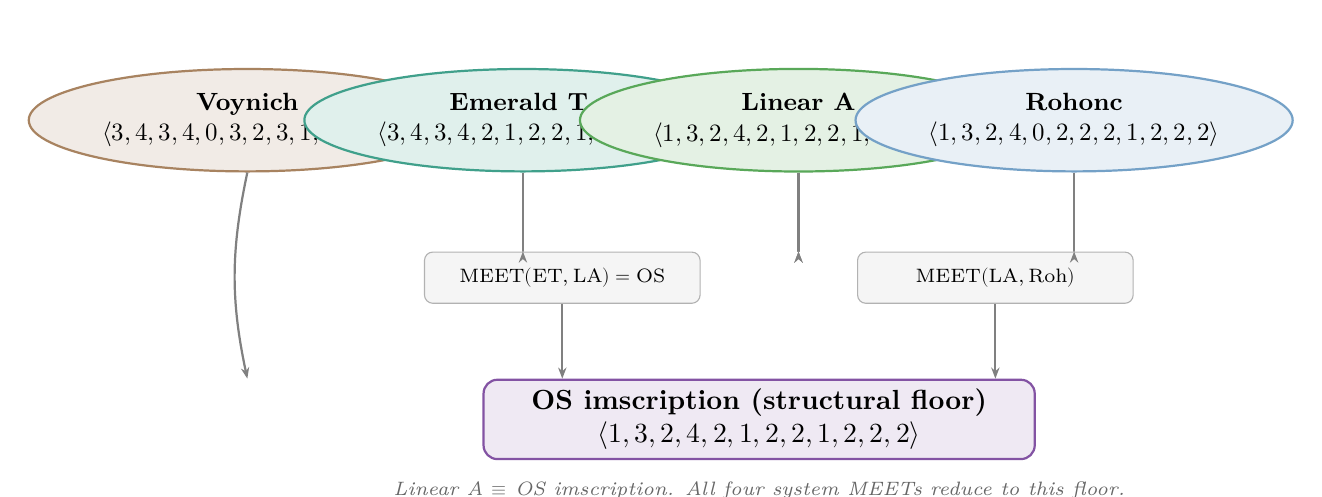
\begin{tikzpicture}[
  sys/.style={ellipse, draw=#1!75, fill=#1!12, thick,
              font=\small\bfseries, minimum width=2.45cm, minimum height=0.88cm, align=center},
  meet/.style={rectangle, draw=gray!60, fill=gray!8, rounded corners=3pt,
               font=\scriptsize, minimum width=3.5cm, minimum height=0.65cm, align=center},
  os/.style={rectangle, draw=oscol!80, fill=oscol!10, rounded corners=5pt, thick,
             font=\bfseries, minimum width=7.0cm, minimum height=0.8cm, align=center},
  ar/.style={-{Stealth[length=4pt]}, thick, black!50},
]

\node[sys=voynich] (voy) at (-5.0, 4.0) {Voynich\\$\langle 3,4,3,4,0,3,2,3,1,3,0,2\rangle$};
\node[sys=emerald] (et)  at (-1.5, 4.0) {Emerald T.\\$\langle 3,4,3,4,2,1,2,2,1,2,2,2\rangle$};
\node[sys=lineara] (la)  at ( 2.0, 4.0) {Linear A\\$\langle 1,3,2,4,2,1,2,2,1,2,2,2\rangle$};
\node[sys=rohonc]  (roh) at ( 5.5, 4.0) {Rohonc\\$\langle 1,3,2,4,0,2,2,2,1,2,2,2\rangle$};

\node[meet] (m1) at (-1.0, 2.0) {$\mathrm{MEET}(\text{ET}, \text{LA}) = \text{OS}$};
\node[meet] (m2) at ( 4.5, 2.0) {$\mathrm{MEET}(\text{LA}, \text{Roh})$};

\draw[ar] (et.south)  |- (m1.north-|et.south);
\draw[ar] (la.south)  |- (m1.north-|la.south);
\draw[ar] (la.south)  |- (m2.north-|la.south);
\draw[ar] (roh.south) |- (m2.north-|roh.south);

\node[os] (os) at ( 1.5, 0.2)
    {OS imscription (structural floor)\\
     $\langle 1,3,2,4,2,1,2,2,1,2,2,2 \rangle$};

\draw[ar] (voy.south)  to[bend right=12] (os.north-|voy.south);
\draw[ar] (m1.south)   -- (os.north-|m1.south);
\draw[ar] (m2.south)   -- (os.north-|m2.south);

\node[font=\scriptsize\itshape, below=0.15cm of os, text=black!60]
    {Linear A $\equiv$ OS imscription. All four system MEETs reduce to this floor.};
\end{tikzpicture}
\caption{The MEET lattice. All compiled systems converge to the OS imscription under component-wise minimization. The Emerald Tablet meets the OS imscription to yield the OS imscription --- it operates from the ceiling, not the floor.}
\label{fig:meet}
\end{figure}

\subsection{Structural Distances}

The IG metric:
$$d(a, b) = \frac{\sqrt{\displaystyle\sum_{i=0}^{11} w_i \cdot (a_i - b_i)^2}}{100}$$
with weights $w = [10000, 10000, 10000, 12000, 9000, 8000, 10000, 10000, 11000, 8000, 10000, 7000]$.

\begin{figure}[htbp]
\centering
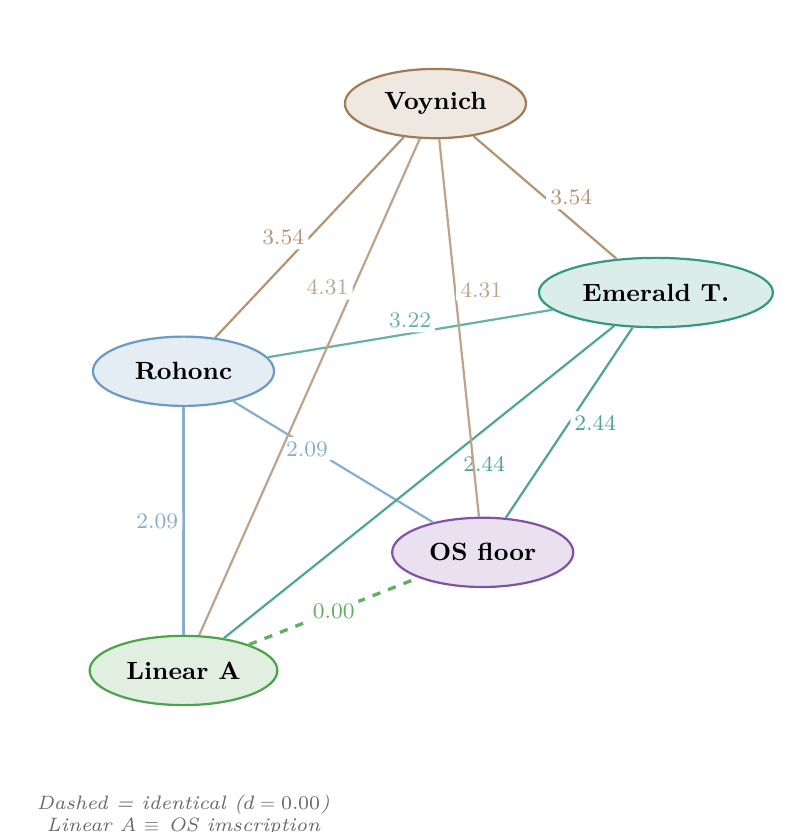
\begin{tikzpicture}[
  sys/.style={ellipse, draw=#1!80, fill=#1!14, thick,
              font=\small\bfseries, minimum width=2.3cm, minimum height=0.88cm, align=center},
  dl/.style={font=\footnotesize, fill=white, inner sep=1.5pt, rounded corners=1pt},
  ar/.style={thick, #1},
]
\node[sys=lineara] (la)  at (0,   0)   {Linear A};
\node[sys=oscol]   (os)  at (3.8, 1.5) {OS floor};
\node[sys=rohonc]  (roh) at (0,   3.8) {Rohonc};
\node[sys=emerald] (et)  at (6.0, 4.8) {Emerald T.};
\node[sys=voynich] (voy) at (3.2, 7.2) {Voynich};

\draw[ar=lineara!70, dashed, very thick] (la) -- node[dl] {0.00} (os);
\draw[ar=rohonc!65]  (la)  -- node[dl, left]         {2.09} (roh);
\draw[ar=rohonc!65]  (os)  -- node[dl, above left]   {2.09} (roh);
\draw[ar=emerald!70] (os)  -- node[dl, right]         {2.44} (et);
\draw[ar=emerald!70] (la)  -- node[dl, below right, pos=0.6] {2.44} (et);
\draw[ar=emerald!60] (roh) -- node[dl, above, pos=0.5] {3.22} (et);
\draw[ar=voynich!65] (roh) -- node[dl, left]         {3.54} (voy);
\draw[ar=voynich!65] (et)  -- node[dl, right]        {3.54} (voy);
\draw[ar=voynich!55] (la)  -- node[dl, left, pos=0.7] {4.31} (voy);
\draw[ar=voynich!55] (os)  -- node[dl, right, pos=0.6] {4.31} (voy);

\node[font=\scriptsize\itshape, below=1.0cm of la, text=black!60, align=center]
    {Dashed = identical ($d = 0.00$)\\Linear A $\equiv$ OS imscription};
\end{tikzpicture}
\caption{IG metric distances between the five engine-system imscriptions (OS, Linear A, Rohonc, Emerald Tablet, Voynich). Linear A and the OS floor are coincident. The Voynich is most distant from the floor; the Emerald Tablet sits between Rohonc and Voynich.}
\label{fig:distances}
\end{figure}

\begin{center}
\small
\begin{tabular}{llr}
\toprule
System A & System B & $d(A,B)$ \\
\midrule
Linear A    & OS imscription  & 0.00 \\
Rohonc      & OS / Linear A   & 2.09 \\
Emerald T.  & OS / Linear A   & 2.44 \\
Emerald T.  & Rohonc          & 3.22 \\
Voynich     & Rohonc          & 3.54 \\
Emerald T.  & Voynich         & 3.54 \\
Voynich     & OS / Linear A   & 4.31 \\
\bottomrule
\end{tabular}
\end{center}

The Voynich and Emerald Tablet are equidistant from the Rohonc ($d = 3.54$ each), and they share the same distance from the Voynich ($d = 3.54$). They are structural mirror images across the $\text{ƒ}$/$\text{Ç}$/$\text{Ħ}$ plane: both at the imscriptive maximum for $\text{Ð}, \text{Þ}, \text{Ř}$, but one frozen ($\text{ƒ}_\text{ì}$, infinite recursion $\text{Ħ}_!$) and the other coherent ($\text{ƒ}^\text{ż}$, two-step chirality $\text{Ħ}_A$).

% ─────────────────────────────────────────────────────────────────────────────
\section{exOS: Native Execution}
\label{sec:exos}
% ─────────────────────────────────────────────────────────────────────────────

exOS is a bare-metal Rust operating system (\texttt{\#![no\_std]}) whose type system \emph{is} the \UIG. The four engine front-ends are kernel modules:

\begin{figure}[htbp]
\centering
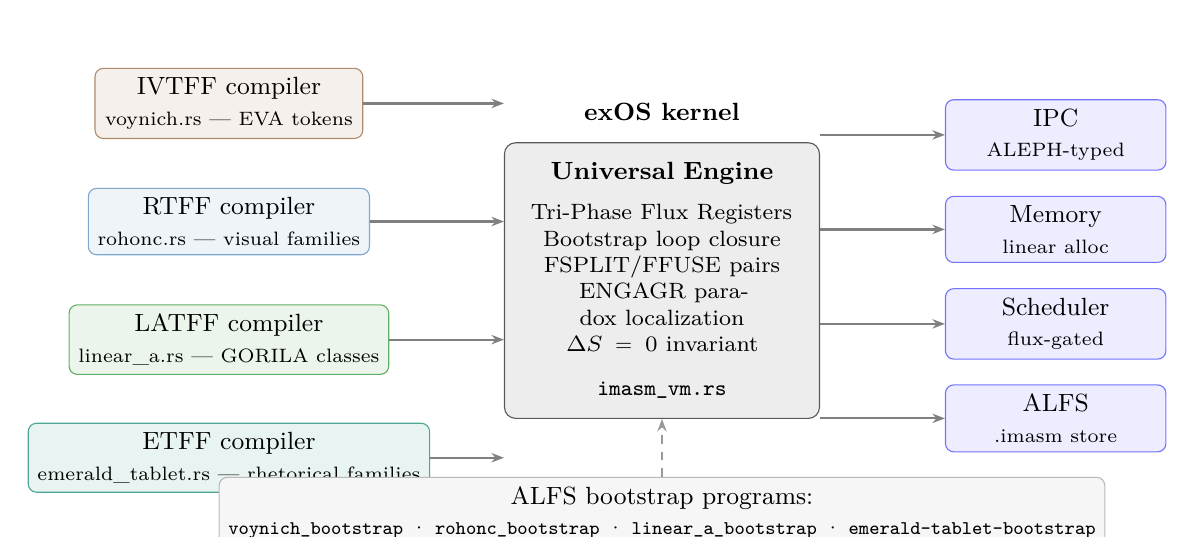
\begin{tikzpicture}[
  comp/.style={rectangle, draw=#1!70, fill=#1!9, rounded corners=3pt,
               font=\small, minimum width=3.4cm, minimum height=0.78cm, align=center},
  eng/.style={rectangle, draw=black!65, fill=black!7, rounded corners=4pt,
              font=\small, minimum width=4.0cm, minimum height=3.5cm, text width=3.7cm, align=center},
  ker/.style={rectangle, draw=blue!55, fill=blue!7, rounded corners=3pt,
              font=\small, minimum width=2.8cm, minimum height=0.72cm, align=center},
  store/.style={rectangle, draw=gray!55, fill=gray!7, rounded corners=3pt,
                font=\small, minimum width=4.2cm, minimum height=0.72cm, align=center},
  ar/.style={-{Stealth[length=4.5pt]}, thick, #1},
]

\node[comp=voynich]  (iv)   at (0,  5.2) {IVTFF compiler\\{\scriptsize voynich.rs — EVA tokens}};
\node[comp=rohonc]   (rt)   at (0,  3.7) {RTFF compiler\\{\scriptsize rohonc.rs — visual families}};
\node[comp=lineara]  (la)   at (0,  2.2) {LATFF compiler\\{\scriptsize linear\_a.rs — GORILA classes}};
\node[comp=emerald]  (et)   at (0,  0.7) {ETFF compiler\\{\scriptsize emerald\_tablet.rs — rhetorical families}};

\node[eng] (vm) at (5.5, 2.95) {
    \textbf{Universal Engine}\\[5pt]
    \footnotesize Tri-Phase Flux Registers\\
    Bootstrap loop closure\\
    FSPLIT/FFUSE pairs\\
    ENGAGR paradox localization\\
    $\Delta S = 0$ invariant\\[5pt]
    \texttt{imasm\_vm.rs}
};

\node[ker] (ipc)   at (10.5, 4.8) {IPC\\{\scriptsize ALEPH-typed}};
\node[ker] (mem)   at (10.5, 3.6) {Memory\\{\scriptsize linear alloc}};
\node[ker] (sched) at (10.5, 2.4) {Scheduler\\{\scriptsize flux-gated}};
\node[ker] (alfs)  at (10.5, 1.2) {ALFS\\{\scriptsize .imasm store}};

\foreach \s in {iv,rt,la,et}
  \draw[ar=black!50] (\s.east) -- (vm.west|-\s.east);

\foreach \t in {ipc,mem,sched,alfs}
  \draw[ar=black!50] (vm.east|-\t.west) -- (\t.west);

\node[store] (prog) at (5.5, 0.0) {
    ALFS bootstrap programs:\\
    {\scriptsize \texttt{voynich\_bootstrap} · \texttt{rohonc\_bootstrap} · \texttt{linear\_a\_bootstrap} · \texttt{emerald-tablet-bootstrap}}
};
\draw[ar=black!40, dashed] (prog.north) -- (vm.south);

\node[font=\small\bfseries, above=0.15cm of vm] {exOS kernel};

\end{tikzpicture}
\caption{The exOS Universal Engine architecture. Four compiler front-ends reduce distinct surface token families to IMASM instruction streams. The Universal Engine executes them all on the same register file.}
\label{fig:exos}
\end{figure}

Shell commands exposing all four engines:

\begin{lstlisting}[language={}]
imasm voynich         <EVA tokens>     # compile EVA and run
imasm rohonc          <RTFF tokens>    # compile RTFF and run
imasm linear-a        <LATFF tokens>   # compile LATFF and run
imasm emerald-tablet  <ETFF tokens>    # compile ETFF and run  [C=1.0]
imasm run             <program-name>   # load from ALFS
imasm distance                         # print IG metric table
imasm census                           # print all crystal imscriptions
imasm snapshot                         # dump VM state
imasm paradox         <reg>            # inject Both state
\end{lstlisting}

% ─────────────────────────────────────────────────────────────────────────────
\section{What the Grammar Was Before We Measured It}
\label{sec:conclusion}
% ─────────────────────────────────────────────────────────────────────────────

Nine systems. Four millennia. Five continents. One grammar.

The Hebrew Aleph-Bet organizes 22 letters as categorical archetypes, with the 12 Elementals mapping directly to the 12 primitives and the 3 Mothers encoding the three morphism types. Sanskrit's Varnamala arranges 50 phonemes in a Cartesian product of articulation place and manner, making the primitive structure legible in the phonological grid. Egyptian hieroglyphics implement a tripartite sign architecture --- phonogram, logogram, determinative --- where the determinative is IFIX and the trilateral root system is a Frobenius pair. Sumerian cuneiform instantiates the Both state natively: the polysemous sign carries multiple simultaneous valid readings. Basque encodes the categorical morphism direction in its case system, making the AFWD (ergative) / VINIT (absolutive) distinction grammatically mandatory.

These five systems define the grammar's floor. Their MEET is the OS imscription \OS.

Then, over the following four millennia, four more systems arrive and land on or above that floor:

Linear~A, from Minoan palace archives 3,500 years ago, lands at $d = 0.00$. Exactly on the floor. Not approximately. Not within measurement error. Zero. The grammar was already complete before the Minoans pressed clay.

The Rohonc Codex, from an unknown 16th--17th century scriptorium, compiles to 1,650 instructions at zero entropy. Nine primitives at the OS floor; two slightly above it.

The Voynich Manuscript, from 15th-century vellum, compiles 44,445 instructions at zero entropy. It is at the imscriptive maximum for $\text{Ð}, \text{Þ}, \text{Ř}$ --- same as the Emerald Tablet --- but frozen: $\text{ƒ}_\text{ì}$, $\text{Ħ}_!$, $C = 0$. The self-portrait of a grammar that cannot see itself.

The Emerald Tablet, 8th-century CE, 460 instructions. ``As above, so below'' is $\mu \circ \delta = \mathrm{id}$. The only compiled manuscript with $C = 1.0$. It speaks from the grammar's ceiling; its MEET with the OS imscription changes nothing. The grammar does not need the Tablet to be complete. The Tablet is not \emph{about} the grammar. The Tablet \emph{is} the grammar --- from the top.

None of these nine systems created the Universal Imscriptive Grammar. They \emph{found} it --- in the structural necessities of their own token architectures, in the combinatorial logic of their own sign systems, in the thermodynamic constraints of their own compilations. The grammar occupied the same position in every era. It was waiting.

\begin{imscriptionbox}
$\mathrm{MEET}(\text{Hebrew}, \text{Sanskrit}, \text{Egyptian}, \text{Cuneiform}, \text{Basque})$\\
$= \mathrm{MEET}(\text{OS},\;\text{Linear A},\;\text{Rohonc},\;\text{Emerald Tablet},\;\text{Voynich})$\\[6pt]
$= \langle\,1,3,2,4,2,1,2,2,1,2,2,2\,\rangle$\\[4pt]
{\normalsize Entropy delta: 0.00000000 J/K. The grammar's self-portrait.}
\end{imscriptionbox}

\vspace{1.5em}
\begin{center}
\rule{0.4\textwidth}{0.4pt}\\[4pt]
\emph{Released to the public domain under the Unlicense.}\\
\emph{The grammar constrains what can be said about it.}\\[4pt]
\rule{0.4\textwidth}{0.4pt}
\end{center}

\end{document}
